

\begin{table}[h]
    \begin{subtable}[h]{0.45\textwidth}
    \begin{tabular}{|c|c|c|}
        \hline
        $m$ (massa) & $l$ (lunghezza) & $k$\\
        \hline

        $(117 \pm 1)\; g$  & $(137.0 \pm 0.5) \;mm$ & $(290 \pm 50)\; Nm^{-1}$\\ 
        $(135 \pm 1)\; g$  & $(129.0 \pm 0.5) \;mm$ & $(220 \pm 30)\; Nm^{-1}$\\ 
        $(249 \pm 1)\; g$  & $(148.0 \pm 0.5) \;mm$ & $(163 \pm 8)\; Nm^{-1}$\\ 
        $(387 \pm 1)\; g$  & $(159.0 \pm 0.5) \;mm$ & $(146 \pm 4)\; Nm^{-1}$\\ 
        $(526 \pm 1)\; g$  & $(173.0 \pm 0.5) \;mm$ & $(129 \pm 2)\; Nm^{-1}$\\ 
        $(623 \pm 1)\; g$  & $(183.0 \pm 0.5) \;mm$ & $(122.2 \pm 1.7)\; Nm^{-1}$\\ 


        \hline
    \end{tabular}
    \end{subtable}
    \hfill
    \begin{subtable}[h]{0.45\textwidth}
        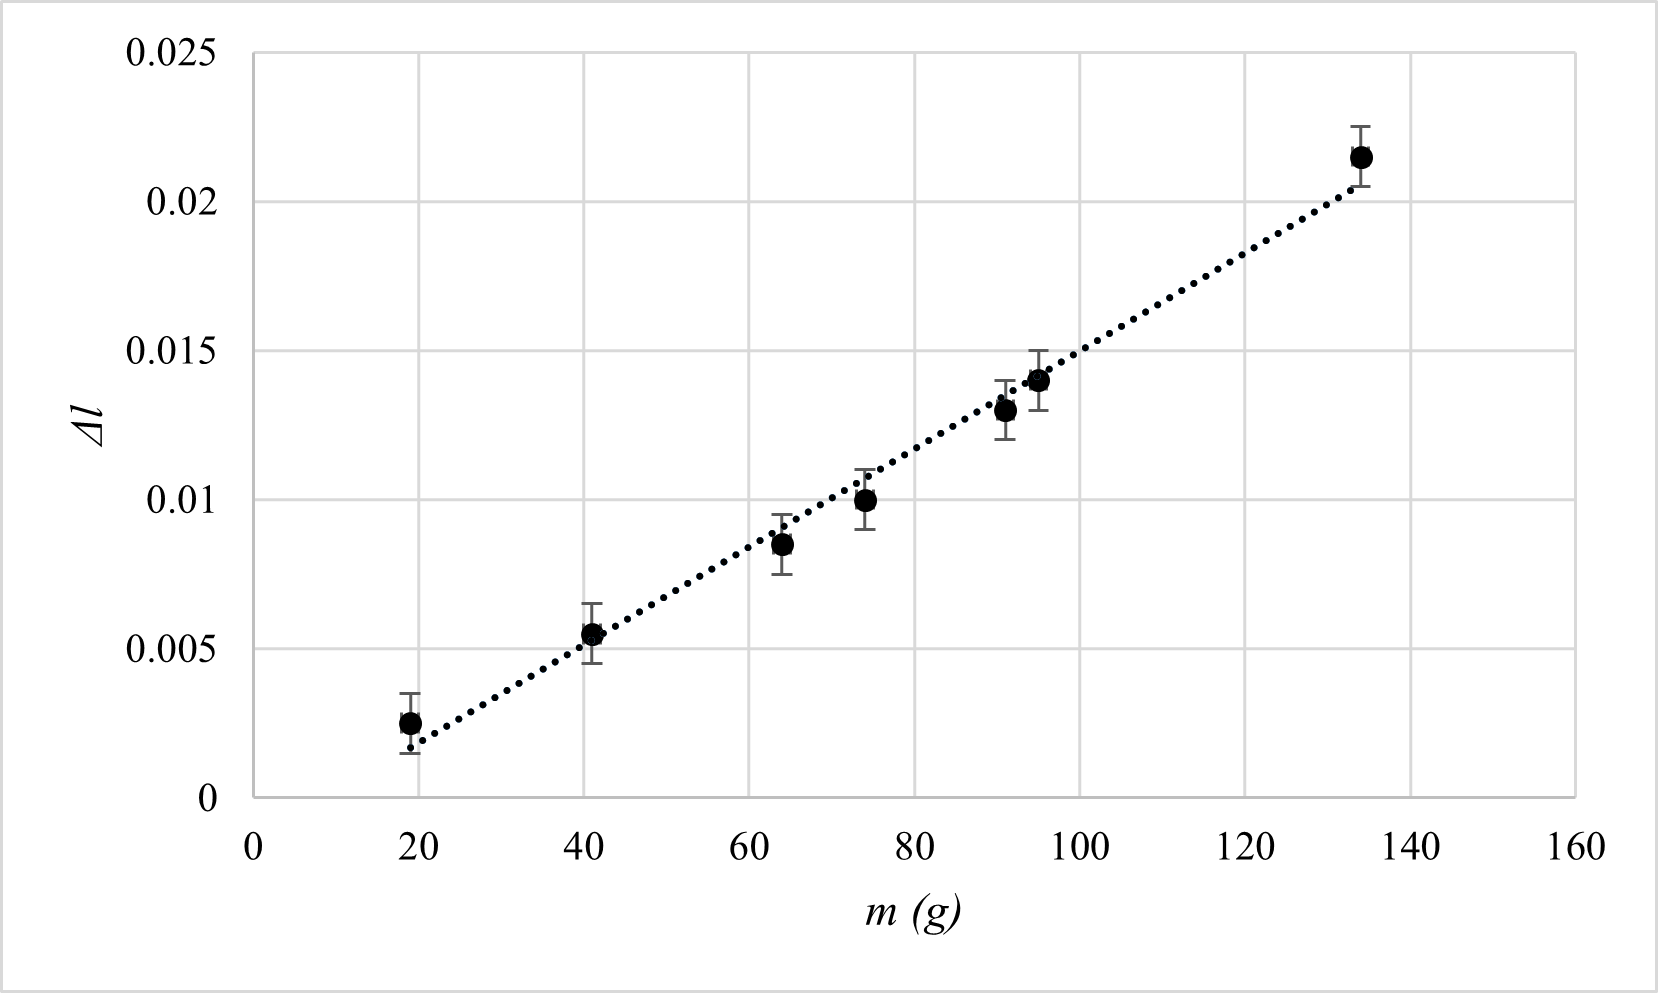
\includegraphics[width = 6cm]{plots/plt2mm.png}
    \end{subtable}
    \caption{Elastico $8\,mm$ ($l_0 = 133.0\, mm \pm 0.5\,mm$) $\qq \sigma_k = 18 \; Nm^{-1}$}
    \label{tabellaElasitco8}
\end{table}
